% \documentclass{book}

\documentclass[12pt]{article}
\usepackage[pdfborder={0 0 0.5 [3 2]}]{hyperref}%
\usepackage[left=1in,right=1in,top=1in,bottom=1in]{geometry}%
\usepackage[shortalphabetic]{amsrefs}%
\usepackage{amsmath}
\usepackage{enumerate}
\usepackage{enumitem}
\usepackage{amssymb}                
\usepackage{amsmath}                
\usepackage{amsfonts}
\usepackage{amsthm}
\usepackage{bbm}
\usepackage[table,xcdraw]{xcolor}
\usepackage{tikz}
\usepackage{float}
\usepackage{svg}
\usepackage{mathtools}
\usepackage{cool}
\usepackage{url}
\usepackage{graphicx,epsfig}
\usepackage{makecell}
\usepackage{array}

\def\noi{\noindent}
\def\T{{\mathbb T}}
\def\R{{\mathbb R}}
\def\N{{\mathbb N}}
\def\C{{\mathbb C}}
\def\Z{{\mathbb Z}}
\def\P{{\mathbb P}}
\def\E{{\mathbb E}}
\def\Q{\mathbb{Q}}
\def\ind{{\mathbb I}}

\def\cale{{\mathcal E}}
\def\cals{{\mathcal S}}
\def\calc{{\mathcal C}}
\def\caln{{\mathcal N}}
\def\calb{{\mathcal B}}
\def\calg{{\cal G}}

\graphicspath{ {images/} }
\renewcommand{\arraystretch}{3}

\begin{document}

\begin{enumerate}
\item (10 points) Let $X$ and $Y$ be continuous random variables with joint probability density given by:
\[
f(x,y) = \begin{cases}
cx & x \geq 0, 0 \leq x^2 \leq y \leq 1 \\
0 & \text{otherwise}
\end{cases}
\]
\begin{enumerate}
\item Find the value of $c$ for which $f(x,y)$ is a valid joint probability density function?\\

First step is to draw a picture of the region, then integrate the joint density over the region and set the integral equal to 1.
\begin{figure}[H]
\centering
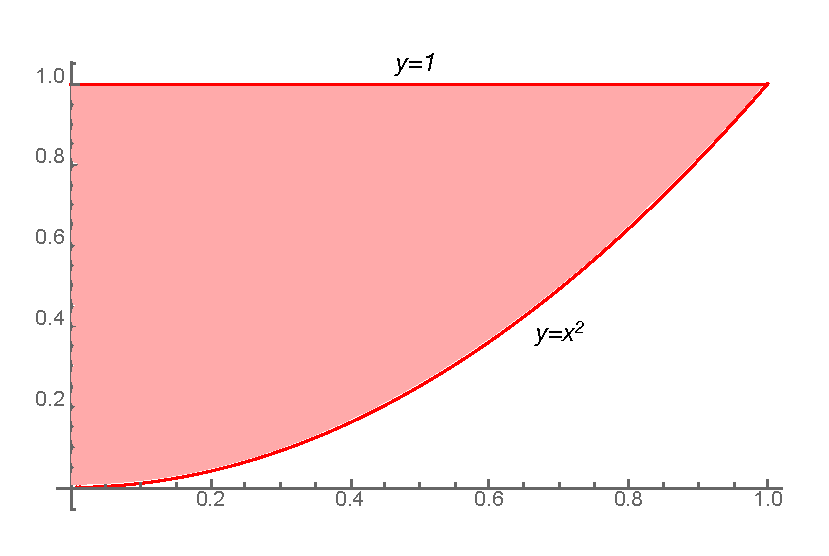
\includegraphics[width=8cm]{exam2region.eps}
\end{figure}
\begin{align*}
1 &= \int_0^1 \int_0^{\sqrt{y}} cx dx dy\\
&= c \int_0^1 \frac{x^2}{2}\Bigr|_0^{\sqrt{y}} dy\\
&= \frac{c}{2} \int_0^1 y dy\\
&= \frac{c}{2}\frac{y^2}{2}\Bigr|_0^1\\
&= \frac{c}{4}
\end{align*}
From this we conclude $c = 4$.

\item Find the expected value of $X$.\\

First we find the marginal density of $X$ by integrating the joint density over $y$.
\begin{align*}
f_X(x) &= \int_{x^2}^1 4x dy\\
&= 4 x y\Bigr|_{x^2}^1 \\
&= 4 x (1 - x^2)\\
&= 4 (x - x^3) 
\end{align*}
The bounds on the marginal density are from 0 to 1. For the expected value,
\begin{align*}
\E(X) &= \int_0^1 x 4(x - x^3) dx\\
&= 4 \int_0^1 (x^2 - x^4) dx\\
&= 4 \left( \frac{x^3}{3} - \frac{x^5}{5} \right)\Bigr|_0^1\\
&= 4 \left( \frac{1}{3} - \frac{1}{5} \right)\\
&= \frac{8}{15}
\end{align*}

\item Find the conditional density of $X$ given $Y = y$. Do not forget to include appropriate bounds for the density function.
\end{enumerate}
First we need the marginal density of $Y$.
\begin{align*}
f_Y(y) &= \int_0^{\sqrt{y}} 4x dx\\
&= 2x^2 \Bigr|_0^{\sqrt{y}} \\
&= 2y
\end{align*}
The bounds on the marginal density are from 0 to 1. For the conditional density, we divide the joint density by the marignal density.
\begin{align*}
f(x|Y = y) &= \frac{4x}{2y}\\
&= 2 \frac{x}{y}
\end{align*}
If $Y = y$, then $X$ can only range from 0 to $\sqrt{y}$, thus we have:
\[
f(x|Y = y) = \begin{cases}
2 \dfrac{x}{y} & 0 \leq x \leq \sqrt{y}\\
0 & \text{otherwise}
\end{cases}
\]

\pagebreak

\item (10 points) You are interested in the proportion $p$ of registered voters in Pennsylvania who prefer Clinton. You take a sample of $n$ voters from the population. Let $Y$ be the number of voters in your sample who prefer Clinton. We showed in class that $Y \sim \text{Binomial}(n, p)$ and that $\hat{p} = \frac{Y}{n}$ is an unbiased estimator for p. The standard estimator for the variance of $Y$ is:
\[
\hat{V} = n \hat{p}(1 - \hat{p}) = n \left( \frac{Y}{n}\right)\left(1 - \frac{Y}{n} \right)
\]
\begin{enumerate}
\item Show that $\hat{V}$ is a biased estimator for the variance of $Y$.\\

\begin{align*}
\E(\hat{V}) &= \E\left[ n \left( \frac{Y}{n}\right)\left(1 - \frac{Y}{n} \right) \right] \\
&= \E\left[Y \left( 1 - \frac{Y}{n} \right) \right] \\
&= \E(Y) - \frac{1}{n} \E(Y^2) 
\end{align*}
By the Magic Variance Formula,
\[
\E(Y^2) = Var(Y) + [\E(Y)]^2
\]
Substituting this in, and using the known expected value and variance of a binomial random variable,
\begin{align*}
\E(\hat{V}) &= \E(Y) - \frac{1}{n} ( Var(Y) + [\E(Y)]^2 )\\
&= np - \frac{1}{n}[np(1-p) + (np)^2]\\
&= np - p(1-p) - np^2 \\
&= p( n - (1 - p) - np) \\
&= p[ n(1 - p) - (1 - p)]\\
&= p[ (n - 1)(1-p) ]\\
&= (n-1)p(1-p)
\end{align*}
Since this is not equal to $Var(Y) = np(1-p)$, this is biased.

\item Modify $\hat{V}$ so that you obtain an unbiased estimator for the variance of $Y$.\\

If we multiply $\hat{V}$ by $\frac{n}{n-1}$, we get an unbiased estimator.
\end{enumerate}
\pagebreak 

\item (10 points) Suppose you choose a point uniformly at random from the interval $[0, 1]$. After you do so, your friend chooses a point uniformly at random between 0 and your point.
\begin{enumerate}
\item Find the joint probability density function of the two points. Do not forget to include appropriate bounds for the density function.\\

Let $X$ be your point, and $Y$ be your friend's point. Then $X \sim $Uniform(0, 1). $Y$, conditioned on $X = x$, is a uniform random variable from $0$ to $x$. Thus we have a marginal density for $X$:
\[
f_X(x) = \begin{cases}
1 & 0 \leq x \leq 1 \\
0 & \text{otherwise}
\end{cases}
\]
And we have a conditional density for $Y$ given $X = x$.
\[
f(y|X=x) = \begin{cases}
\dfrac{1}{x} & 0 \leq y \leq x \\
0 & \text{otherwise}
\end{cases}
\]
Since the joint density is the product of the conditional and the marginal densities, we have:
\[
f(x, y) = \begin{cases}
\dfrac{1}{x} & 0 \leq y \leq x \leq 1 \\
0 & \text{otherwise}
\end{cases}
\]
You could also reason your way to this result by drawing a picture and coming up with a density with the desired properties.
\item What is the expected value of the product of the two points?
\end{enumerate}
\begin{align*}
\E(XY) &= \int_0^1 \int_0^x xy \frac{1}{x} dy dx \\
&= \int_0^1 \int_0^x y dy dx \\
&= \int_0^1 \frac{y^2}{2}\Bigr|_0^x dx\\
&= \frac{1}{2} \int_0^1 \frac{x^2} dx \\
&= \frac{1}{2} \frac{x^3}{3}\Bigr|_0^1 \\
&= \frac{1}{6}
\end{align*}

\pagebreak 

\item (10 points) During study breaks from APMA 1650, you play Pok\'emon GO. The average number of Pok\'emon a player catches in a 30-minute period is 6. Assume that Pok\'emon are caught independently from each other.
\begin{enumerate}
\item Suppose you just caught a Pok\'emon. Modeling this with an appropriate probability distribution, what is the probability that it will take less than 10 minutes for you to catch your next Pok\'emon? 

Let $X$ be the time it takes to catch a new Pok\'emon. Since the average number of Pok\'emon caught in one minute is $6/30 = 1/5$, let $X \sim $ Exponential(1/5). Then
\begin{align*}
\P(0 \leq X \leq 10) &= \int_0^{10} \frac{1}{5}e^{-(1/5)x} dx \\
&= -e^{-(1/5)x}\Bigr|_0^10 \\
&= -e^{-10/5} - (-1) \\
&= 1 - e^{-2}
\end{align*}
\item Being a good statistician, you decide to play Pok\'emon Go long enough to catch 100 more Pok\'emon. You measure the amount of time it takes to catch each of the 100 Pok\'emon and compute the sample mean. What is the probability that this sample mean is between 4 and 6 minutes?\\

By the Central Limit Theorem, the sample $\bar{X}$ is a normal distirbution. The population is exponential with mean 5 and variance $5^2$, so the population standard deviation is 5. (This can all be looked up in the reference table). Then the mean of $\bar{X}$ is 5 and the standard deviation of $\bar{X}$ is $5/\sqrt{100} = 1/2$. Thus $\bar{X}\sim $ Normal(5, 1/2).
\begin{align*}
\P(4 < \bar{X} < 6) &= \P\left( \frac{4-5}{1/2} < Z < \frac{5-6}{1/2} \right) \\
&= \P( -2 < Z < 2 )\\
&= 0.9722 - 0.0228
\end{align*}
\end{enumerate}
You could also have used the 68-95-99.7 rule since we want the probability of being within 2 standard deviations of the mean.
\pagebreak

\item (10 points) Despite being sleep-deprived from all the Pok\'emon you caught in the previous problem, you decide to continue playing Pok\'emon GO. Once again, the average number of Pok\'emon a player catches in a 30-minute period is 6, and Pok\'emon are caught independently from each other.
\begin{enumerate}
\item Modeling this with an appropriate probability distribution, what is the probability that you catch 1 or fewer Pok\'emon in a 10-minute period?\\

Let $Y$ be the number of Pok\'emon caught in a 10-minute period. The average number of Pok\'emon caught in a 10-minute period is $6/3 = 2$, so let $Y \sim $ Poisson(2). Then
\begin{align*}
\P(Y \leq 1) &= \P(Y = 0) + \P(Y = 1) \\
&= \frac{e^{-2} 2^0}{0!} + \frac{e^{-2} 2^1}{1!} \\
&= 3 e^{-2}
\end{align*}

\item Your friend, who also plays Pok\'emon GO, claims to have caught more than 4 (i.e. 5 or more) Pok\'emon in a 10-minute period. Can you be at least 75\% certain that your friend is lying? Justify your answer mathematically. This does not require a calculator.\\

By Chebyshev's Inequality, since the mean and variance of $Y$ is 2,
\begin{align*}
\P(Y \geq 5) &\leq \P( |Y - 2| \geq 3) \\
&\leq \frac{Var(Y)}{3^2} \\
&=\frac{2}{9} < \frac{1}{4} = 0.25
\end{align*}
\end{enumerate}
Since the probability that $Y \leq 5$ is less than or equal to 0.25, you can be at least 75\% certain that your friend is lying.\\

If you use Markov's Inequality, you get:
\[
\P(Y \geq 5) \leq \frac{\E(Y)}{5} = \frac{2}{5} = 0.40
\] 
which is unfortunately not good enough. The moral of the story is that Markov's inequality is not very good, so in cases where you know the variance (like you do here), you want to use Chebyshev's Inequality.
\end{enumerate}

\end{document}

